% Created 2022-08-22 Mon 14:22
% Intended LaTeX compiler: pdflatex
\documentclass[11pt]{article}
\usepackage[utf8]{inputenc}
\usepackage[T1]{fontenc}
\usepackage{graphicx}
\usepackage{longtable}
\usepackage{wrapfig}
\usepackage{rotating}
\usepackage[normalem]{ulem}
\usepackage{amsmath}
\usepackage{amssymb}
\usepackage{capt-of}
\usepackage{hyperref}
\author{Vincent Toups}
\date{\today}
\title{}
\hypersetup{
 pdfauthor={Vincent Toups},
 pdftitle={},
 pdfkeywords={},
 pdfsubject={},
 pdfcreator={Emacs 28.1 (Org mode 9.5.2)}, 
 pdflang={English}}
\begin{document}

\tableofcontents

\section{Why Learn Unix}
\label{sec:org85e601e}

Unix, generally in the form of Linux, but also commonly encountered as
the underlying idiom of OSX and other important systems, powers the
world.

\begin{table}[htbp]
\label{tab:org0c517c8}
\centering
\begin{tabular}{llrrr}
Source & Month & Year & Unix & Windows\\
\hline
W3Techs & May & 2021 & 75.3 & 24.8\\
W3Techs & Jan & 2020 & 71.0 & 29.0\\
W3Techs & Jan & 2018 & 66.8 & 33.2\\
W3Techs & Jan & 2016 & 67.7 & 32.3\\
W3Techs & Jan & 2014 & 66.8 & 33.2\\
W3Techs & Jan & 2012 & 63.5 & 36.5\\
\end{tabular}
\end{table}

\begin{verbatim}
library(tidyverse);
print(ggplot(servers, aes(Year, Unix)) + geom_line());
\end{verbatim}

And the result: 

\begin{figure}[htbp]
\centering
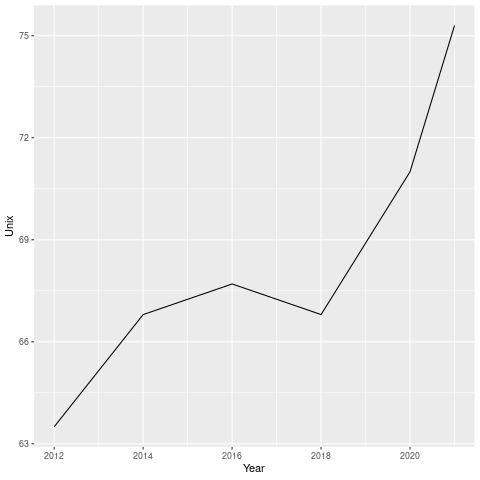
\includegraphics[width=.9\linewidth]{./z.png}
\caption{\label{fig:orgedb295c}Percentage of servers running unix like operating systems over time.}
\end{figure}

Some very popular data science software (RStudio Server, Jupyter/Labs)
runs on Linux (even if you access them via a web browser on any
platform).

This means that if you become a working data scientist or want to
support yourself working with many data scientific tools as a
researcher, some knowledge of Unix will be useful to you.

If that weren't enough, the true key to portable data science is
Docker. It is true that you can run Docker in Windows but the
configuration of docker containers requires a good working knowledge
of the Unix idiom, since most containers are Linux based.

For this book, Linux based Docker Containers will be the norm. For
Windows users I highly recommend using the instructions located \href{https://docs.docker.com/docker-for-windows/wsl/}{here}:

\begin{verbatim}
https://docs.docker.com/docker-for-windows/wsl/
\end{verbatim}

to set up both Windows Subsystem for Linux (which will allow you to
run a Linux environment natively on Windows) and setting up the
appropriate Docker install on top of it. 

Mac users can use the standard Docker install. Linux users will
typically know what they want to do, but the short version is install
Docker via the instructions appropriate to your distribution and make
sure you are in the docker group. 

Will will discuss Docker in greater detail in later chapters.

\section{Introduction to Computers}
\label{sec:orgc650e00}

If you were born after 1990 or so there is a good chance you've never
seen a text-based shell. Modern computers of the most common variety
(smartphones) do an even more aggressive (or successful, depending on
your attitude and needs) job of protecting you from the underlying
operating system. Thus it is worth a brief conceptual review:

A computer, even a smartphone, is a machine with a processor, which
performs mathematical operations on data, memory, which is volatile
storage (it will be erased in the event that the computer is turned
off) which forms the short term memory of the machine, and
non-volatile storage (disks, solid state memory, even, sometimes
still, spinning rust) which is persistant data store which survives
even when the machine is off.

At the most basic level, a computer reads data from a disk into local
memory and its processor reads a program out of that memory, executing
instructions which modify the data in memory and/or write it back to
long term storage.

In the early days of computing this was the conceptual world the
compute programmer inhabited as well: interacting with a computer was
the process of telling it, in great detail, which memory to access,
what to do with it, and how to store or output the results.

Since those days the trend has been towards even greater levels of
abstraction.  Now, a typical smartphone "protects" the user from most
of these details: you never think explicitly, about the distinctions
between storage and memory or about the details of how programs work.

\section{How to Understand Computer Languages}
\label{sec:org06ec6f0}

A programming language is a program which takes text (represented as a
"string" of characters) and \uline{interprets} it to produce some sort of
value or side effect.

In order to understand a computer programming language you need to
build a model of this process in your mind. The process of
transforming text into values and actions is called "evaluation" or
"interpretation" in the lingo of computer science and as we learn to
get around in the shell we will need to accumulate a set of
"evaluation rules" in our mind. The more rules we accumulate the more
we will understand shell scripting.

When we get to learning R and Python the same process will apply.

\section{Introduction to Unix Shells}
\label{sec:org355eab2}

We will now dive much deeper into the computer than you may have
before. What may be surprising about this jump is just how much more
water there is beneath us still: Unix Shells, while providing what
must seem like shockingly low level access to the workings of a
machine compared to modern graphical user interfaces, still afford us
an almost entirely abstract representation of our computer, albiet one
which has traded implicitness for explicitness to a great degree.

A shell (in this context) is a textual interface between you and the
services provided by your operating system. From the shell we can do
all the things we ordinarily do from a graphical user interface:
inspect files, launch programs, organize data, poke and peek at
various system resources and settings. We do these things by executing
commands.

Before we dive into the details you might ask yourself: why would we
\uline{want} to have such low level access? It is true, these text-mode
shells impose a substantial cognitive burden on the user, particularly
at first. What do we purchase with that additional cognitive energy?

\begin{enumerate}
\item control - the shell gives us enormous, fine grained, control over
the resources the computer gives us.
\item reproducibility - because all the actions we might undertake with
the shell are represented as text, we can easily copy and paste
them into a file and re-run them.
\end{enumerate}

\subsection{Running a Shell}
\label{sec:orgc3f3d66}

If you are on Linux or OSX you will want to run your Terminal
application. If you are working on a Windows machine you may want to
install Git Bash, Cygwin, or install Ubuntu or another Linux variant
in a Virtual Machine or spin up an Ubuntu container in Docker.

\subsection{Control}
\label{sec:orgf059413}

The unix Shell is loosely organized under the banner of "The Unix
Philosophy". Whereas graphical user interfaces tend to become
monoliths from which it is difficult to escape, the Unix Philosophy
suggests that tools (programs) should:

\begin{enumerate}
\item do one thing
\item do it well
\end{enumerate}

This philosophy is enabled by a very simple organizational principal:
almost everything in Unix is represented as a file. All programs
operate on files, typically by reading an input file and producing an
output file. More complex outcomes are acheived by stringing many
small programs together, each operating on the output of the previous
until a desired result occurs. Text based files are very commonly the
inputs and outputs of these processes.

\subsection{Reproducibility}
\label{sec:org635c84b}

Unix Shells are text based interfaces. While it can seem onerous,
initially, to have to laborously type out each desired command to the
shell, doing so is very traceable. After we understand what we want to
do by interacting with a shell directly, we can copy and paste the
commands we've concocted into a "shell script" and re-execute
them. Repeatative tasks can be trialed a few times and then run over
and over again and gradually refined. 

When you combine this fact with tools like git, which make it easy to
record the history of a file over time, you have system for ensuring
that what you do is recorded for posterity and reproducible. 

Graphical User Interfaces, in contrast, introduce many non-meaningful
degrees of freedom (for instance, the precise x, y coordinate of a
folder on your desktop) which make it difficult to automate workflows
for them, even when such tools exist. 

Learning to use the Shell will teach you a powerful way of simple and
easily orchestrating work your computer does.

\section{Shell Concepts}
\label{sec:org42082e9}

\subsection{Many Shells}
\label{sec:orga9e1078}

Unix supports \uline{many} different shells which behave
similarly. Throughout this course I will be assuming \href{https://en.wikipedia.org/wiki/Bash\_(Unix\_shell)}{bash} because it
is the most common. I'll be trying to write bash code which will run
in most other shells (most notably zsh, which is recently the default
OSX shell) for simplicity. But if you run into an issue, make sure you
are running bash by simply typing:

\begin{verbatim}
bash
\end{verbatim}
\captionof{figure}{how to start bash}

\subsection{Types of Data}
\label{sec:org0024568}

\begin{enumerate}
\item Strings: an ordered collection of characters.
\item Numbers
\end{enumerate}

On the shell things tend to pass back and forth between these types
pretty fluently. This is bad design but we have to live with it.

The most important thing to bear in mind is that when I say something
is "just a string" I mean that the computer doesn't know what to do
with it - its just purely data.

\subsection{REPL}
\label{sec:orgb2d5c2f}

The shell is one example of a "read, eval, print" loop. It 

\begin{enumerate}
\item reads an input (typically a line of text)
\item evaluates it (turning it into an action or side effect or value of
some sort)
\item and then prints the result (or nothing, if a side effect)
\end{enumerate}

At its most superficial level this is how we interact with a shell:

\begin{verbatim}
ls
\end{verbatim}

\begin{verbatim}
4.png
experiment.sh
homework.md
missfont.log
my-commands
solutions.md
unix.html
unix.log
unix.org
unix.tex
z.pdf
z.png
\end{verbatim}

Reading is trivial - the input you type is just a list of
characters. Evaluation is where things get tricky:

\subsection{Evaluation}
\label{sec:org81b7c39}

A theme of this course is that \uline{all programming languages} do more or
less the same thing: they translate text into actions. If you develop
a good mental model of that process then you \uline{understand} the
language.

Given the ubiquity of Bash, its evaluation model is surprisingly
complicated. Luckily for us, we will be concerned with its simplest
aspects.

Superficially and in the simplest case, bash does the following when
you type a command:

\begin{enumerate}
\item the text is split into tokens on the spaces
\item the first token is assumed to be a command you want to
execute. Bash tries to find a file which implements this command by
looking it up on the "PATH" (of which more later).
\item the subsequent tokens are passed to the command as
"arguments". Arguments are additional pieces of information the
command may want or need to change the way it executes.
\end{enumerate}

So when we typed "ls" above, bash read this as us wanting to run the
command "ls" which it found on our hard drive. Then it saw that we
passed no arguments to the command, so it executed it without any.

\subsubsection{Eg 1}
\label{sec:org2bfc435}

\begin{verbatim}
ls -t -l
\end{verbatim}

\begin{verbatim}
total 204
-rw-r--r-- 1 toups toups 76559 Aug 22 14:22 unix.html
-rw-r--r-- 1 toups toups 32052 Aug 22 14:17 unix.org
-rw-r--r-- 1 toups toups   859 Jul  6 10:56 homework.md
-rw-r--r-- 1 toups toups   933 Jun  9 13:55 solutions.md
drwxr-xr-x 2 toups toups  4096 May 17 14:19 my-commands
-rw-r--r-- 1 toups toups  6534 May 17 14:19 4.png
-rw-r--r-- 1 toups toups   130 May 17 14:19 experiment.sh
-rw-r--r-- 1 toups toups    54 May 17 14:19 missfont.log
-rw-r--r-- 1 toups toups  3202 May 17 14:19 unix.log
-rw-r--r-- 1 toups toups 39925 May 17 14:19 unix.tex
-rw-r--r-- 1 toups toups 12641 May 17 14:19 z.pdf
-rw-r--r-- 1 toups toups  7457 May 17 14:19 z.png
\end{verbatim}

In the above example, the shell reads "ls -t -l", splits it apart on
the spaces like this: \texttt{[ls, -t, -l]} finds the \texttt{ls} command, and
passes the \texttt{-t} and \texttt{-l} arguments to it. Note that these arguments
are just passed as strings to the \texttt{ls} command. It is up to \texttt{ls} to
decide what, if anything, they mean. In this case, they mean "sort the
file list by modification time" (\texttt{-t}) and "print out more information
about the files" (\texttt{-l})

\subsubsection{Eg 2}
\label{sec:org3b1e426}

\begin{verbatim}
#something_silly a b c
\end{verbatim}

The above will generate an error like this:

\begin{verbatim}
bash: line 1: something_silly: command not found
\end{verbatim}

\subsection{The PATH and other environment variables}
\label{sec:org9d05fcc}

When a string is evaluated the shell must find what command we want to
run. How does it do so? 

Some background: apart from a few built in commands (the so-called
\href{https://www.gnu.org/software/bash/manual/html\_node/Bash-Builtins.html}{builtins}) commands in shell scripts are just executable files stored
somewhere on the hard drive.  The command \texttt{which} tells us where such
commands qua files are located:


\begin{verbatim}
which which
\end{verbatim}

\begin{verbatim}
/usr/bin/which
\end{verbatim}


A good piece of jargon to have in your head here is that \texttt{which}
"resolves" to \texttt{/usr/bin/which}.

If you haven't seen unix style file locations, note:

\begin{enumerate}
\item on a unix system \uline{every file} lives beneath the so-called "root" of
the file system, called \texttt{/}.
\item anything between two \texttt{/} (called \uline{path separators}) is a
\_directory.
\item the last term may be a directory or a file. In this case, it is the
executable file which implements the \texttt{which} commands.
\end{enumerate}

\texttt{which} resolves in the same way that Bash resolves, but how does that
work?

They look  in something called an environment variable called
PATH. You can see what an environment variable holds like this:

\begin{verbatim}
echo $PATH
\end{verbatim}

\begin{verbatim}
/home/toups/.local/bin:/usr/local/sbin:/usr/local/bin:/usr/bin:/var/lib/flatpak/exports/bin:/usr/bin/site_perl:/usr/bin/vendor_perl:/usr/bin/core_perl:/var/lib/snapd/snap/bin
\end{verbatim}

To understand this behavior we need to add a new rule to our mental
"evaluation engine":

\phantomsection
\label{orgbf44417}
\begin{quote}
When we see a \$ followed immediately by a name we look up the value of
the variable named and insert it into the string. This happens before
the other rules are executed.
\end{quote}

Apparently, \texttt{PATH} contains a series of locations on the filesystem
separated by ":" characters. Bash searches this list in order to find
executables during command evaluation.

So in the case of \texttt{which} it looks in 

\begin{enumerate}
\item \texttt{/home/toups/.local/bin} (no hit)
\item \texttt{/usr/local/local/sbin} (no hit)
\item \texttt{/usr/bin} (hit!)
\end{enumerate}

By modifying this environment variable we can modify the way bash
looks up commands. But how would we create our own command to test out
this ability?

Let's create a directory

And then let's create a directory:

\begin{verbatim}
mkdir my-commands
readlink -f my-commands
\end{verbatim}

\begin{verbatim}
/home/toups/work/courses/bios611/lectures/02-unix/my-commands
\end{verbatim}

(your file will obviously be somewhere else on your personal computer).

And now lets create the file

\begin{verbatim}
#!/bin/bash

echo hello world

\end{verbatim}
\captionof{figure}{my-commands/hello.sh}

We can do this with this shell magic

\begin{verbatim}

  cat <<EOF > my-commands/hello.sh
echo hello world
EOF

\end{verbatim}

First we need to tell our Unix that we want to give the file
"hello.sh" permission to act as an executable:

\begin{verbatim}
chmod u+x my-commands/hello.sh
\end{verbatim}

And then we can 

\begin{verbatim}
PATH="$(readlink -f my-commands):$PATH"
hello.sh
\end{verbatim}

\begin{verbatim}
hello world
\end{verbatim}

In order to understand this result we need to add another rule:

\phantomsection
\label{orgdb8dc30}
\begin{quote}
If we see a name followed immediate by an equal sign and then a value,
modify or create a new environment variable of that name with the
specified value. No regular evaluation occurs but environment
variables themselves are expanded before setting the value.
\end{quote}

If some of the above steps are a little confusing to you, that is ok -
we're not going for a full understanding of working on the command
line: we want just enough to get around.

We will develop more as we go.

The PATH isn't the only environment variable. What variables are
defined will vary a lot by system and situation, but you can see a
list of all of them by saying:

\begin{verbatim}
env | head
\end{verbatim}
\captionof{figure}{\label{orgd9b561a}the environment}

\begin{verbatim}
SHELL=/bin/bash
SESSION_MANAGER=local/work-arch:@/tmp/.ICE-unix/847,unix/work-arch:/tmp/.ICE-unix/847
WINDOWID=100663303
QT_SCREEN_SCALE_FACTORS=eDP-1=1;DP-1=1;HDMI-1=1;DP-2=1;
COLORTERM=truecolor
XDG_CONFIG_DIRS=/home/toups/.config/kdedefaults:/etc/xdg
XDG_SESSION_PATH=/org/freedesktop/DisplayManager/Session1
LANGUAGE=
LC_ADDRESS=en_US.UTF-8
LC_NAME=en_US.UTF-8
\end{verbatim}

\subsection{Variables}
\label{sec:org2484487}

You can declare your own variables or modify those that already exist
(assuming they aren't read only).

The easiest way to declare a variable is:

\begin{verbatim}
VARNAME=somevalue
echo $VARNAME
\end{verbatim}
\captionof{figure}{\label{org8f69f4d}declaring a variable}

\begin{verbatim}
somevalue
\end{verbatim}

Note that when we declare a variable we do \uline{not} precede the name with
a \texttt{\$}. The dollar sign is what tells Bash to look the variable value
up when we want to \uline{use} it somewhere. 

With variable definition and usage rules in our head, we can now
extend our mental model of bash evaluation.

\begin{enumerate}
\item for every line in a script
a. perform variable substitution (wherever we see a \$NAME look up
the value and insert it into the line)
b. if the line is a command, do command evaluation
   otherwise do variable assignment
\end{enumerate}

The only really important remaining ingredient is non-variable
substitution.

Consider again the following line from the above example:

\begin{verbatim}
PATH="$(readlink -f my-commands):$PATH"
\end{verbatim}
\captionof{figure}{\label{org8e0aba3}Substitution}

Ordinarily no \uline{evaluation} occurs on the right hand side of an
assignment. The material there is just treated as a string (or a
number, if it happens to be a number). But by using a \texttt{\$(...)}
construct we can perform a substitution: the interior of the \texttt{\$(...)}
is evaluated like a command and the result is inserted into the line
where it appears.

We can use this to compose together multiple commands. Consider that
\texttt{ls -t | head -n 1} will return the most recently modified file. \texttt{head
<filename>} will print out the first few lines of a file. If we want
to print the first few lines of the most recently modified file:

\begin{verbatim}
head $(ls -t | head -n 1)
\end{verbatim}
\captionof{figure}{\label{org9c63f13}combining commands with substitution}

\begin{verbatim}
<?xml version="1.0" encoding="utf-8"?>
<!DOCTYPE html PUBLIC "-//W3C//DTD XHTML 1.0 Strict//EN"
"http://www.w3.org/TR/xhtml1/DTD/xhtml1-strict.dtd">
<html xmlns="http://www.w3.org/1999/xhtml" lang="en" xml:lang="en">
<head>
<!-- 2022-08-22 Mon 14:22 -->
<meta http-equiv="Content-Type" content="text/html;charset=utf-8" />
<meta name="viewport" content="width=device-width, initial-scale=1" />
<title>&lrm;</title>
<meta name="author" content="Vincent Toups" />
\end{verbatim}

(The most recently modified file is this document!).

\subsection{stdin, stdout, stderr and pipes}
\label{sec:orgebfffad}

We have one more important element of the shell to learn. Recall that
shell commands communicate by reading input from somewhere and writing
it out to a new location. Most often the place they read from is the
"standard input" (abbreviated stdin). And the most common place they
output things is the "standard output". If there is an error of some
kind most processes report this on another file called the "standard
error."

In the above example, when we used the command \texttt{head} we passed a
filename in as a command line argument and the result was printed to
the standard output.

We can also redirect the standard output to a file:

\begin{verbatim}
ls -t > files-in-order
head files-in-order -n 3
rm files-in-order
\end{verbatim}
\captionof{figure}{\label{org682d778}Redirecting the standard output.}

\begin{verbatim}
files-in-order
unix.html
unix.org
\end{verbatim}

The syntax \texttt{<COMMAND> > file} sends the standard output to \texttt{file}.

But often creating a temporary file is a hassle if we just want to
apply many commands in sequence. Thus we can also "pipe" one command's
output to another's input. In that case the second command reads from
the output of the previous \uline{instead} of from the stdin file.

\begin{verbatim}
ls -t | head -n 3
\end{verbatim}
\captionof{figure}{\label{org6394c95}Piping output into input.}

\begin{verbatim}
unix.html
unix.org
homework.md
\end{verbatim}

The \texttt{|} (called a "pipe") means: take the output from the first item
and send it to the second. We can pipe many times in a row.

\begin{verbatim}
ls -t | head -n 3 | grep y
\end{verbatim}
\captionof{figure}{\label{orgcac20c8}A chain of pipes.}

The output of \texttt{ls} goes to \texttt{head} and the output of \texttt{head} goes to
\texttt{grep}. Some bash scripts are little more than a long series of
pipes. Learning to program this way is very enlightening and we'll see
a similar "chain of operations" approach in R and Python.

\subsection{Conventions to bear in mind}
\label{sec:orgc9ef043}

The shell itself doesn't enforce any convention whatsoever on the
arguments passed to a command. Each space separated collection of
characters counts as an argument and a command may interpret them
in any way it wishes.

However, there are some conventions that you'll typically see.

\subsubsection{The sub-command pattern}
\label{sec:orgd311d54}

Many of the tools we'll use in this course will use the
sub-command pattern. In this pattern a command will implement a
set of sub-commands. These are typically invoked by mentioning the
command and then the sub-command without any prefixes. For
example:

\begin{verbatim}
git status
\end{verbatim}

Invokes the \texttt{status} sub-command of the command
\texttt{git}. Sub-commands can and often do take additional arguments
which are treated just like any other shell argument.

\begin{verbatim}
git diff --stat
\end{verbatim}

In this case the \texttt{-{}-stat} is a command line switch, something
which we recognize as modifying the behavior of the command.

\subsubsection{short and long options}
\label{sec:org2946f5e}

Command line arguments are also given in the form of short and
long options.

A short option is written as \texttt{-<single-letter>} and a long option
is written \texttt{-{}-<option-name>}. It is often the case (but not
always) that a short option has a long option which represents the
same thing and vice versa. For example

\begin{verbatim}
ls -a
\end{verbatim}

and

\begin{verbatim}
ls --all 
\end{verbatim}

mean the same thing. Options can take inputs, which just means one
or more tokens after the option without \texttt{-} or \texttt{-{}-} in front of
them.

For instance:

\begin{verbatim}
head -n 10 hello.txt
\end{verbatim}

In the above example "10" is an argument to the \texttt{-n} option. In
this case it tells \texttt{head} that we want to print the first 10 lines
of the file \texttt{hello.txt}.

It is often the case that any arguments at the end of the argument
list not preceeded by options that take arguments are files that
the command operates on or otherwise creates or modifies.

\begin{verbatim}
ln -s hello.txt link-to-hello.txt
\end{verbatim}

Here \texttt{-s} is a switch which takes no arguments and the last two
arguments to the command are interpreted as the source and target
of the \texttt{ln} command itself.

\subsubsection{Warning}
\label{sec:org31b5a48}

Not every shell command will follow these conventions. In
particular, \texttt{find} lets you specify \emph{long} arguments with a single
\texttt{-} in front of them. But keeping these conventions in mind will
help you understand what is happening on the shell.

\subsection{Important Commands}
\label{sec:org9b1ec0f}

\subsubsection{man}
\label{sec:org1e7cbe1}

Short for "manual" - given a command name it returns information about
using that command. Some commands are not documented this way but
almost all the most common ones are.

\begin{verbatim}
man bash | head -n 10
\end{verbatim}
\captionof{figure}{\label{org267d0cd}Using man.}

\begin{verbatim}
BASH(1)                     General Commands Manual                    BASH(1)

NAME
       bash - GNU Bourne-Again SHell

SYNOPSIS
       bash [options] [command_string | file]

COPYRIGHT
       Bash is Copyright (C) 1989-2020 by the Free Software Foundation, Inc.
\end{verbatim}

I consult a man page at least once a day while working so don't be
afraid to lean on this command.

\subsubsection{apropos}
\label{sec:orged62698}

\texttt{apropos} takes a keyword and returns a list of commands that might be
related. Also handy if you are new to a system, although these days
google is probably more effective. Sometimes handy in a pinch, though.

\begin{verbatim}
apropos lisp
\end{verbatim}
\captionof{figure}{\label{org7e488f6}Using apropos.}

\begin{verbatim}
ecl (1)              - Embeddable Common Lisp
ecl-config (1)       - Embeddable Common Lisp configuration query
maxima (1)           - Common Lisp version of MACSYMA symbolic mathematics pa...
sbcl (1)             - Steel Bank Common Lisp
\end{verbatim}

\subsubsection{cd \& pwd}
\label{sec:orge2dba8b}

\texttt{cd} changes the current working directory and \texttt{pwd} tells you the
current working directory.

\begin{verbatim}
OLD_DIR=$(pwd)
cd /tmp # the temporary directory on a Linux machine.
touch test # touch just creates an empty file or updates a file's modification time.
cd $OLD_DIR
\end{verbatim}
\captionof{figure}{\label{org7e6828f}cd example.}

Also interesting: \texttt{pushd} and \texttt{popd}.

\subsubsection{find}
\label{sec:orgd4229e2}

\texttt{find} lets us search for files in a variety of ways. A simple
example:

\begin{verbatim}
find . -iname "*.png"
\end{verbatim}
\captionof{figure}{\label{orgb97e4f1}Finding all R files beneath the pwd.}

\begin{verbatim}
./z.png
./4.png
\end{verbatim}

\texttt{find} is very powerful and also a little weird in places. But it is
so useful that having a basic working knowledge of the command will be
very much worth it.

\subsubsection{grep}
\label{sec:org609876a}

\texttt{grep} lets you search for things \uline{in} files:

\begin{verbatim}
grep -n hello unix.*
\end{verbatim}
\captionof{figure}{\label{org33fbcef}Using grep.}

\begin{verbatim}
unix.html:896:<label class="org-src-name"><span class="listing-number">Listing 2: </span>my-commands/hello.sh</label><pre class="src src-bash"><span style="color: #b22222;">#</span><span style="color: #b22222;">!/bin/</span><span style="color: #0000cd;">bash</span>
unix.html:898:<span style="color: #b35caf;">echo</span> hello world
unix.html:909:  cat &lt;&lt;EOF &gt; my-commands/hello.sh
unix.html:910:<span style="color: #ffa54f;">echo hello world</span>
unix.html:924:"hello.sh" permission to act as an executable:
unix.html:928:<pre class="src src-sh">chmod u+x my-commands/hello.sh
unix.html:944:hello.sh
unix.html:949:<pre class="src src-sh">hello world
unix.html:1273:<pre class="src src-bash">head -n 10 hello.txt
unix.html:1280:of the file <code>hello.txt</code>.
unix.html:1290:<pre class="src src-bash">ln -s hello.txt link-to-hello.txt
unix.html:1440:<label class="org-src-name"><span class="listing-number">Listing 14: </span>Using grep.</label><pre class="src src-bash" id="org6f128bc">grep -n hello unix.*
unix.html:1445:<pre class="src src-org">unix.html:895:&lt;label class="org-src-name"&gt;&lt;span class="listing-number"&gt;Listing 2: &lt;/span&gt;my-commands/hello.sh&lt;/label&gt;&lt;pre class="src src-bash"&gt;&lt;span style="color: #cd853f;"&gt;#&lt;/span&gt;&lt;span style="color: #cd853f;"&gt;!/bin/&lt;/span&gt;&lt;span style="color: #20b2aa; font-weight: bold;"&gt;bash&lt;/span&gt;
unix.html:1446:unix.html:897:&lt;span style="color: #76ee00;"&gt;echo&lt;/span&gt; hello world
unix.html:1447:unix.html:908:  cat &amp;lt;&amp;lt;EOF &amp;gt; my-commands/hello.sh
unix.html:1448:unix.html:909:&lt;span style="color: #ffff00; font-weight: bold;"&gt;echo hello world&lt;/span&gt;
unix.html:1449:unix.html:923:"hello.sh" permission to act as an executable:
unix.html:1450:unix.html:927:&lt;pre class="src src-sh"&gt;chmod u+x my-commands/hello.sh
unix.html:1451:unix.html:943:hello.sh
unix.html:1452:unix.html:948:&lt;pre class="src src-sh"&gt;hello world
unix.html:1453:unix.html:1259:&lt;pre class="src src-bash"&gt;head -n 10 hello.txt
unix.html:1454:unix.html:1266:of the file &lt;code&gt;hello.txt&lt;/code&gt;.
unix.html:1455:unix.html:1276:&lt;pre class="src src-bash"&gt;ln -s hello.txt link-to-hello.txt
unix.html:1456:unix.html:1418:&lt;label class="org-src-name"&gt;&lt;span class="listing-number"&gt;Listing 14: &lt;/span&gt;Using grep.&lt;/label&gt;&lt;pre class="src src-bash" id="orgf4537c2"&gt;grep -n hello unix.*
unix.html:1457:unix.html:1423:&lt;pre class="src src-org"&gt;unix.html:887:&amp;lt;label class="org-src-name"&amp;gt;&amp;lt;span class="listing-number"&amp;gt;Listing 4: &amp;lt;/span&amp;gt;my-commands/hello.sh&amp;lt;/label&amp;gt;&amp;lt;pre class="src src-bash"&amp;gt;&amp;lt;span style="color: #cd853f;"&amp;gt;#&amp;lt;/span&amp;gt;&amp;lt;span style="color: #cd853f;"&amp;gt;!/bin/&amp;lt;/span&amp;gt;&amp;lt;span style="color: #20b2aa; font-weight: bold;"&amp;gt;bash&amp;lt;/span&amp;gt;
unix.html:1458:unix.html:1424:unix.html:889:&amp;lt;span style="color: #76ee00;"&amp;gt;echo&amp;lt;/span&amp;gt; hello world
unix.html:1459:unix.html:1425:unix.html:896:"hello.sh" permission to act as an executable:
unix.html:1460:unix.html:1426:unix.html:900:&amp;lt;pre class="src src-bash"&amp;gt;chmod u+x my-commands/hello.sh
unix.html:1461:unix.html:1427:unix.html:911:hello.sh
unix.html:1462:unix.html:1428:unix.html:916:&amp;lt;pre class="src src-org"&amp;gt;hello world
unix.html:1463:unix.html:1429:unix.html:1227:&amp;lt;pre class="src src-bash"&amp;gt;head -n 10 hello.txt
unix.html:1464:unix.html:1430:unix.html:1234:of the file &amp;lt;code&amp;gt;hello.txt&amp;lt;/code&amp;gt;.
unix.html:1465:unix.html:1431:unix.html:1244:&amp;lt;pre class="src src-bash"&amp;gt;ln -s hello.txt link-to-hello.txt
unix.html:1466:unix.html:1432:unix.html:1386:&amp;lt;label class="org-src-name"&amp;gt;&amp;lt;span class="listing-number"&amp;gt;Listing 17: &amp;lt;/span&amp;gt;Using grep.&amp;lt;/label&amp;gt;&amp;lt;pre class="src src-bash" id="org832d784"&amp;gt;grep -n hello unix.*
unix.html:1467:unix.html:1433:unix.html:1391:&amp;lt;pre class="src src-org"&amp;gt;unix.html:776:&amp;amp;lt;label class="org-src-name"&amp;amp;gt;&amp;amp;lt;span class="listing-number"&amp;amp;gt;Listing 6: &amp;amp;lt;/span&amp;amp;gt;my-commands/hello.sh&amp;amp;lt;/label&amp;amp;gt;&amp;amp;lt;pre class="src src-bash"&amp;amp;gt;&amp;amp;lt;span style="color: #7f7f7f;"&amp;amp;gt;#&amp;amp;lt;/span&amp;amp;gt;&amp;amp;lt;span style="color: #7f7f7f;"&amp;amp;gt;!/bin/&amp;amp;lt;/span&amp;amp;gt;&amp;amp;lt;span style="color: #1c86ee;"&amp;amp;gt;bash&amp;amp;lt;/span&amp;amp;gt;
unix.html:1468:unix.html:1434:unix.html:1392:unix.html:778:&amp;amp;lt;span style="color: #cd6600;"&amp;amp;gt;echo&amp;amp;lt;/span&amp;amp;gt; hello world
unix.html:1469:unix.html:1435:unix.html:1393:unix.html:785:"hello.sh" permission to act as an executable:
unix.html:1470:unix.html:1436:unix.html:1394:unix.html:789:&amp;amp;lt;pre class="src src-bash"&amp;amp;gt;chmod u+x my-commands/hello.sh
unix.html:1471:unix.html:1437:unix.html:1395:unix.html:799:hello.sh
unix.html:1472:unix.html:1438:unix.html:1396:unix.html:808:hello world
unix.html:1473:unix.html:1439:unix.html:1397:unix.org:365:#+CAPTION: my-commands/hello.sh
unix.html:1474:unix.html:1440:unix.html:1398:unix.org:369:echo hello world
unix.html:1475:unix.html:1441:unix.html:1399:unix.org:374:"hello.sh" permission to act as an executable:
unix.html:1476:unix.html:1442:unix.html:1400:unix.org:377:chmod u+x my-commands/hello.sh
unix.html:1477:unix.html:1443:unix.html:1401:unix.org:389:hello.sh
unix.html:1478:unix.html:1444:unix.html:1402:unix.org:394:hello world
unix.html:1479:unix.html:1445:unix.html:1403:unix.org:628:      head -n 10 hello.txt
unix.html:1480:unix.html:1446:unix.html:1404:unix.org:633:    of the file &amp;lt;span style="color: #b3b3b3;"&amp;gt;~hello.txt~&amp;lt;/span&amp;gt;.
unix.html:1481:unix.html:1447:unix.html:1405:unix.org:640:      ln -s hello.txt link-to-hello.txt
unix.html:1482:unix.html:1448:unix.html:1406:unix.org:749:grep -n hello unix.*
unix.html:1483:unix.html:1449:unix.html:1407:unix.org:754:unix.html:776:&amp;amp;lt;label class="org-src-name"&amp;amp;gt;&amp;amp;lt;span class="listing-number"&amp;amp;gt;Listing 6: &amp;amp;lt;/span&amp;amp;gt;my-commands/hello.sh&amp;amp;lt;/label&amp;amp;gt;&amp;amp;lt;pre class="src src-bash"&amp;amp;gt;&amp;amp;lt;span style="color: #7f7f7f;"&amp;amp;gt;#&amp;amp;lt;/span&amp;amp;gt;&amp;amp;lt;span style="color: #7f7f7f;"&amp;amp;gt;!/bin/&amp;amp;lt;/span&amp;amp;gt;&amp;amp;lt;span style="color: #1c86ee;"&amp;amp;gt;bash&amp;amp;lt;/span&amp;amp;gt;
unix.html:1484:unix.html:1450:unix.html:1408:unix.org:755:unix.html:778:&amp;amp;lt;span style="color: #cd6600;"&amp;amp;gt;echo&amp;amp;lt;/span&amp;amp;gt; hello world
unix.html:1485:unix.html:1451:unix.html:1409:unix.org:756:unix.html:785:"hello.sh" permission to act as an executable:
unix.html:1486:unix.html:1452:unix.html:1410:unix.org:757:unix.html:789:&amp;amp;lt;pre class="src src-bash"&amp;amp;gt;chmod u+x my-commands/hello.sh
unix.html:1487:unix.html:1453:unix.html:1411:unix.org:758:unix.html:799:hello.sh
unix.html:1488:unix.html:1454:unix.html:1412:unix.org:759:unix.html:808:hello world
unix.html:1489:unix.html:1455:unix.html:1413:unix.org:760:unix.org:344:#+CAPTION: my-commands/hello.sh
unix.html:1490:unix.html:1456:unix.html:1414:unix.org:761:unix.org:348:echo hello world
unix.html:1491:unix.html:1457:unix.html:1415:unix.org:762:unix.org:353:"hello.sh" permission to act as an executable:
unix.html:1492:unix.html:1458:unix.html:1416:unix.org:763:unix.org:356:chmod u+x my-commands/hello.sh
unix.html:1493:unix.html:1459:unix.html:1417:unix.org:764:unix.org:368:hello.sh
unix.html:1494:unix.html:1460:unix.html:1418:unix.org:765:unix.org:373:hello world
unix.html:1495:unix.html:1461:unix.html:1419:unix.org:766:unix.org:643:grep hello 
unix.html:1496:unix.html:1462:unix.org:369:#+CAPTION: my-commands/hello.sh
unix.html:1497:unix.html:1463:unix.org:373:echo hello world
unix.html:1498:unix.html:1464:unix.org:381:  cat &amp;lt;&amp;lt;EOF &amp;gt; my-commands/hello.sh
unix.html:1499:unix.html:1465:unix.org:382:echo hello world
unix.html:1500:unix.html:1466:unix.org:393:"hello.sh" permission to act as an executable:
unix.html:1501:unix.html:1467:unix.org:396:chmod u+x my-commands/hello.sh
unix.html:1502:unix.html:1468:unix.org:404:hello.sh
unix.html:1503:unix.html:1469:unix.org:409:hello world
unix.html:1504:unix.html:1470:unix.org:643:      head -n 10 hello.txt
unix.html:1505:unix.html:1471:unix.org:648:    of the file &lt;span style="color: #b3b3b3;"&gt;~hello.txt~&lt;/span&gt;.
unix.html:1506:unix.html:1472:unix.org:655:      ln -s hello.txt link-to-hello.txt
unix.html:1507:unix.html:1473:unix.org:764:grep -n hello unix.*
unix.html:1508:unix.html:1474:unix.org:769:unix.html:776:&amp;lt;label class="org-src-name"&amp;gt;&amp;lt;span class="listing-number"&amp;gt;Listing 6: &amp;lt;/span&amp;gt;my-commands/hello.sh&amp;lt;/label&amp;gt;&amp;lt;pre class="src src-bash"&amp;gt;&amp;lt;span style="color: #7f7f7f;"&amp;gt;#&amp;lt;/span&amp;gt;&amp;lt;span style="color: #7f7f7f;"&amp;gt;!/bin/&amp;lt;/span&amp;gt;&amp;lt;span style="color: #1c86ee;"&amp;gt;bash&amp;lt;/span&amp;gt;
unix.html:1509:unix.html:1475:unix.org:770:unix.html:778:&amp;lt;span style="color: #cd6600;"&amp;gt;echo&amp;lt;/span&amp;gt; hello world
unix.html:1510:unix.html:1476:unix.org:771:unix.html:785:"hello.sh" permission to act as an executable:
unix.html:1511:unix.html:1477:unix.org:772:unix.html:789:&amp;lt;pre class="src src-bash"&amp;gt;chmod u+x my-commands/hello.sh
unix.html:1512:unix.html:1478:unix.org:773:unix.html:799:hello.sh
unix.html:1513:unix.html:1479:unix.org:774:unix.html:808:hello world
unix.html:1514:unix.html:1480:unix.org:775:unix.org:344:#+CAPTION: my-commands/hello.sh
unix.html:1515:unix.html:1481:unix.org:776:unix.org:348:echo hello world
unix.html:1516:unix.html:1482:unix.org:777:unix.org:353:"hello.sh" permission to act as an executable:
unix.html:1517:unix.html:1483:unix.org:778:unix.org:356:chmod u+x my-commands/hello.sh
unix.html:1518:unix.html:1484:unix.org:779:unix.org:368:hello.sh
unix.html:1519:unix.html:1485:unix.org:780:unix.org:373:hello world
unix.html:1520:unix.html:1486:unix.org:781:unix.org:643:grep hello 
unix.html:1521:unix.org:395:#+CAPTION: my-commands/hello.sh
unix.html:1522:unix.org:399:echo hello world
unix.html:1523:unix.org:407:  cat &lt;&lt;EOF &gt; my-commands/hello.sh
unix.html:1524:unix.org:408:echo hello world
unix.html:1525:unix.org:419:"hello.sh" permission to act as an executable:
unix.html:1526:unix.org:422:chmod u+x my-commands/hello.sh
unix.html:1527:unix.org:430:hello.sh
unix.html:1528:unix.org:435:hello world
unix.html:1529:unix.org:679:      head -n 10 hello.txt
unix.html:1530:unix.org:684:    of the file <span style="color: #7f7f7f;">~hello.txt~</span>.
unix.html:1531:unix.org:691:      ln -s hello.txt link-to-hello.txt
unix.html:1532:unix.org:800:grep -n hello unix.*
unix.html:1533:unix.org:805:unix.html:776:&lt;label class="org-src-name"&gt;&lt;span class="listing-number"&gt;Listing 6: &lt;/span&gt;my-commands/hello.sh&lt;/label&gt;&lt;pre class="src src-bash"&gt;&lt;span style="color: #7f7f7f;"&gt;#&lt;/span&gt;&lt;span style="color: #7f7f7f;"&gt;!/bin/&lt;/span&gt;&lt;span style="color: #1c86ee;"&gt;bash&lt;/span&gt;
unix.html:1534:unix.org:806:unix.html:778:&lt;span style="color: #cd6600;"&gt;echo&lt;/span&gt; hello world
unix.html:1535:unix.org:807:unix.html:785:"hello.sh" permission to act as an executable:
unix.html:1536:unix.org:808:unix.html:789:&lt;pre class="src src-bash"&gt;chmod u+x my-commands/hello.sh
unix.html:1537:unix.org:809:unix.html:799:hello.sh
unix.html:1538:unix.org:810:unix.html:808:hello world
unix.html:1539:unix.org:811:unix.org:344:#+CAPTION: my-commands/hello.sh
unix.html:1540:unix.org:812:unix.org:348:echo hello world
unix.html:1541:unix.org:813:unix.org:353:"hello.sh" permission to act as an executable:
unix.html:1542:unix.org:814:unix.org:356:chmod u+x my-commands/hello.sh
unix.html:1543:unix.org:815:unix.org:368:hello.sh
unix.html:1544:unix.org:816:unix.org:373:hello world
unix.html:1545:unix.org:817:unix.org:643:grep hello 
unix.html:1546:unix.tex:435:echo hello world
unix.html:1547:unix.tex:438:\captionof{figure}{my-commands/hello.sh}
unix.html:1548:unix.tex:444:  cat &lt;&lt;EOF &gt; my-commands/hello.sh
unix.html:1549:unix.tex:445:echo hello world
unix.html:1550:unix.tex:451:"hello.sh" permission to act as an executable:
unix.html:1551:unix.tex:454:chmod u+x my-commands/hello.sh
unix.html:1552:unix.tex:461:hello.sh
unix.html:1553:unix.tex:465:hello world
unix.html:1554:unix.tex:563:alias hello="echo hello world"
unix.html:1555:unix.tex:564:hello
unix.html:1556:unix.tex:694:head -n 10 hello.txt
unix.html:1557:unix.tex:699:of the file \texttt{hello.txt}.
unix.html:1558:unix.tex:706:ln -s hello.txt link-to-hello.txt
unix.html:1559:unix.tex:801:grep -n hello unix.*
unix.html:1560:unix.tex:806:unix.html:895:&lt;label class="org-src-name"&gt;&lt;span class="listing-number"&gt;Listing 2: &lt;/span&gt;my-commands/hello.sh&lt;/label&gt;&lt;pre class="src src-bash"&gt;&lt;span style="color: #cd853f;"&gt;#&lt;/span&gt;&lt;span style="color: #cd853f;"&gt;!/bin/&lt;/span&gt;&lt;span style="color: #20b2aa; font-weight: bold;"&gt;bash&lt;/span&gt;
unix.html:1561:unix.tex:807:unix.html:897:&lt;span style="color: #76ee00;"&gt;echo&lt;/span&gt; hello world
unix.html:1562:unix.tex:808:unix.html:908:  cat &amp;lt;&amp;lt;EOF &amp;gt; my-commands/hello.sh
unix.html:1563:unix.tex:809:unix.html:909:&lt;span style="color: #ffff00; font-weight: bold;"&gt;echo hello world&lt;/span&gt;
unix.html:1564:unix.tex:810:unix.html:923:"hello.sh" permission to act as an executable:
unix.html:1565:unix.tex:811:unix.html:927:&lt;pre class="src src-sh"&gt;chmod u+x my-commands/hello.sh
unix.html:1566:unix.tex:812:unix.html:943:hello.sh
unix.html:1567:unix.tex:813:unix.html:948:&lt;pre class="src src-sh"&gt;hello world
unix.html:1568:unix.tex:814:unix.html:1259:&lt;pre class="src src-bash"&gt;head -n 10 hello.txt
unix.html:1569:unix.tex:815:unix.html:1266:of the file &lt;code&gt;hello.txt&lt;/code&gt;.
unix.html:1570:unix.tex:816:unix.html:1276:&lt;pre class="src src-bash"&gt;ln -s hello.txt link-to-hello.txt
unix.html:1571:unix.tex:817:unix.html:1418:&lt;label class="org-src-name"&gt;&lt;span class="listing-number"&gt;Listing 14: &lt;/span&gt;Using grep.&lt;/label&gt;&lt;pre class="src src-bash" id="orgf4537c2"&gt;grep -n hello unix.*
unix.html:1572:unix.tex:818:unix.html:1423:&lt;pre class="src src-org"&gt;unix.html:887:&amp;lt;label class="org-src-name"&amp;gt;&amp;lt;span class="listing-number"&amp;gt;Listing 4: &amp;lt;/span&amp;gt;my-commands/hello.sh&amp;lt;/label&amp;gt;&amp;lt;pre class="src src-bash"&amp;gt;&amp;lt;span style="color: #cd853f;"&amp;gt;#&amp;lt;/span&amp;gt;&amp;lt;span style="color: #cd853f;"&amp;gt;!/bin/&amp;lt;/span&amp;gt;&amp;lt;span style="color: #20b2aa; font-weight: bold;"&amp;gt;bash&amp;lt;/span&amp;gt;
unix.html:1573:unix.tex:819:unix.html:1424:unix.html:889:&amp;lt;span style="color: #76ee00;"&amp;gt;echo&amp;lt;/span&amp;gt; hello world
unix.html:1574:unix.tex:820:unix.html:1425:unix.html:896:"hello.sh" permission to act as an executable:
unix.html:1575:unix.tex:821:unix.html:1426:unix.html:900:&amp;lt;pre class="src src-bash"&amp;gt;chmod u+x my-commands/hello.sh
unix.html:1576:unix.tex:822:unix.html:1427:unix.html:911:hello.sh
unix.html:1577:unix.tex:823:unix.html:1428:unix.html:916:&amp;lt;pre class="src src-org"&amp;gt;hello world
unix.html:1578:unix.tex:824:unix.html:1429:unix.html:1227:&amp;lt;pre class="src src-bash"&amp;gt;head -n 10 hello.txt
unix.html:1579:unix.tex:825:unix.html:1430:unix.html:1234:of the file &amp;lt;code&amp;gt;hello.txt&amp;lt;/code&amp;gt;.
unix.html:1580:unix.tex:826:unix.html:1431:unix.html:1244:&amp;lt;pre class="src src-bash"&amp;gt;ln -s hello.txt link-to-hello.txt
unix.html:1581:unix.tex:827:unix.html:1432:unix.html:1386:&amp;lt;label class="org-src-name"&amp;gt;&amp;lt;span class="listing-number"&amp;gt;Listing 17: &amp;lt;/span&amp;gt;Using grep.&amp;lt;/label&amp;gt;&amp;lt;pre class="src src-bash" id="org832d784"&amp;gt;grep -n hello unix.*
unix.html:1582:unix.tex:828:unix.html:1433:unix.html:1391:&amp;lt;pre class="src src-org"&amp;gt;unix.html:776:&amp;amp;lt;label class="org-src-name"&amp;amp;gt;&amp;amp;lt;span class="listing-number"&amp;amp;gt;Listing 6: &amp;amp;lt;/span&amp;amp;gt;my-commands/hello.sh&amp;amp;lt;/label&amp;amp;gt;&amp;amp;lt;pre class="src src-bash"&amp;amp;gt;&amp;amp;lt;span style="color: #7f7f7f;"&amp;amp;gt;#&amp;amp;lt;/span&amp;amp;gt;&amp;amp;lt;span style="color: #7f7f7f;"&amp;amp;gt;!/bin/&amp;amp;lt;/span&amp;amp;gt;&amp;amp;lt;span style="color: #1c86ee;"&amp;amp;gt;bash&amp;amp;lt;/span&amp;amp;gt;
unix.html:1583:unix.tex:829:unix.html:1434:unix.html:1392:unix.html:778:&amp;amp;lt;span style="color: #cd6600;"&amp;amp;gt;echo&amp;amp;lt;/span&amp;amp;gt; hello world
unix.html:1584:unix.tex:830:unix.html:1435:unix.html:1393:unix.html:785:"hello.sh" permission to act as an executable:
unix.html:1585:unix.tex:831:unix.html:1436:unix.html:1394:unix.html:789:&amp;amp;lt;pre class="src src-bash"&amp;amp;gt;chmod u+x my-commands/hello.sh
unix.html:1586:unix.tex:832:unix.html:1437:unix.html:1395:unix.html:799:hello.sh
unix.html:1587:unix.tex:833:unix.html:1438:unix.html:1396:unix.html:808:hello world
unix.html:1588:unix.tex:834:unix.html:1439:unix.html:1397:unix.org:365:#+CAPTION: my-commands/hello.sh
unix.html:1589:unix.tex:835:unix.html:1440:unix.html:1398:unix.org:369:echo hello world
unix.html:1590:unix.tex:836:unix.html:1441:unix.html:1399:unix.org:374:"hello.sh" permission to act as an executable:
unix.html:1591:unix.tex:837:unix.html:1442:unix.html:1400:unix.org:377:chmod u+x my-commands/hello.sh
unix.html:1592:unix.tex:838:unix.html:1443:unix.html:1401:unix.org:389:hello.sh
unix.html:1593:unix.tex:839:unix.html:1444:unix.html:1402:unix.org:394:hello world
unix.html:1594:unix.tex:840:unix.html:1445:unix.html:1403:unix.org:628:      head -n 10 hello.txt
unix.html:1595:unix.tex:841:unix.html:1446:unix.html:1404:unix.org:633:    of the file &amp;lt;span style="color: #b3b3b3;"&amp;gt;~hello.txt~&amp;lt;/span&amp;gt;.
unix.html:1596:unix.tex:842:unix.html:1447:unix.html:1405:unix.org:640:      ln -s hello.txt link-to-hello.txt
unix.html:1597:unix.tex:843:unix.html:1448:unix.html:1406:unix.org:749:grep -n hello unix.*
unix.html:1598:unix.tex:844:unix.html:1449:unix.html:1407:unix.org:754:unix.html:776:&amp;amp;lt;label class="org-src-name"&amp;amp;gt;&amp;amp;lt;span class="listing-number"&amp;amp;gt;Listing 6: &amp;amp;lt;/span&amp;amp;gt;my-commands/hello.sh&amp;amp;lt;/label&amp;amp;gt;&amp;amp;lt;pre class="src src-bash"&amp;amp;gt;&amp;amp;lt;span style="color: #7f7f7f;"&amp;amp;gt;#&amp;amp;lt;/span&amp;amp;gt;&amp;amp;lt;span style="color: #7f7f7f;"&amp;amp;gt;!/bin/&amp;amp;lt;/span&amp;amp;gt;&amp;amp;lt;span style="color: #1c86ee;"&amp;amp;gt;bash&amp;amp;lt;/span&amp;amp;gt;
unix.html:1599:unix.tex:845:unix.html:1450:unix.html:1408:unix.org:755:unix.html:778:&amp;amp;lt;span style="color: #cd6600;"&amp;amp;gt;echo&amp;amp;lt;/span&amp;amp;gt; hello world
unix.html:1600:unix.tex:846:unix.html:1451:unix.html:1409:unix.org:756:unix.html:785:"hello.sh" permission to act as an executable:
unix.html:1601:unix.tex:847:unix.html:1452:unix.html:1410:unix.org:757:unix.html:789:&amp;amp;lt;pre class="src src-bash"&amp;amp;gt;chmod u+x my-commands/hello.sh
unix.html:1602:unix.tex:848:unix.html:1453:unix.html:1411:unix.org:758:unix.html:799:hello.sh
unix.html:1603:unix.tex:849:unix.html:1454:unix.html:1412:unix.org:759:unix.html:808:hello world
unix.html:1604:unix.tex:850:unix.html:1455:unix.html:1413:unix.org:760:unix.org:344:#+CAPTION: my-commands/hello.sh
unix.html:1605:unix.tex:851:unix.html:1456:unix.html:1414:unix.org:761:unix.org:348:echo hello world
unix.html:1606:unix.tex:852:unix.html:1457:unix.html:1415:unix.org:762:unix.org:353:"hello.sh" permission to act as an executable:
unix.html:1607:unix.tex:853:unix.html:1458:unix.html:1416:unix.org:763:unix.org:356:chmod u+x my-commands/hello.sh
unix.html:1608:unix.tex:854:unix.html:1459:unix.html:1417:unix.org:764:unix.org:368:hello.sh
unix.html:1609:unix.tex:855:unix.html:1460:unix.html:1418:unix.org:765:unix.org:373:hello world
unix.html:1610:unix.tex:856:unix.html:1461:unix.html:1419:unix.org:766:unix.org:643:grep hello 
unix.html:1611:unix.tex:857:unix.html:1462:unix.org:369:#+CAPTION: my-commands/hello.sh
unix.html:1612:unix.tex:858:unix.html:1463:unix.org:373:echo hello world
unix.html:1613:unix.tex:859:unix.html:1464:unix.org:381:  cat &amp;lt;&amp;lt;EOF &amp;gt; my-commands/hello.sh
unix.html:1614:unix.tex:860:unix.html:1465:unix.org:382:echo hello world
unix.html:1615:unix.tex:861:unix.html:1466:unix.org:393:"hello.sh" permission to act as an executable:
unix.html:1616:unix.tex:862:unix.html:1467:unix.org:396:chmod u+x my-commands/hello.sh
unix.html:1617:unix.tex:863:unix.html:1468:unix.org:404:hello.sh
unix.html:1618:unix.tex:864:unix.html:1469:unix.org:409:hello world
unix.html:1619:unix.tex:865:unix.html:1470:unix.org:643:      head -n 10 hello.txt
unix.html:1620:unix.tex:866:unix.html:1471:unix.org:648:    of the file &lt;span style="color: #b3b3b3;"&gt;~hello.txt~&lt;/span&gt;.
unix.html:1621:unix.tex:867:unix.html:1472:unix.org:655:      ln -s hello.txt link-to-hello.txt
unix.html:1622:unix.tex:868:unix.html:1473:unix.org:764:grep -n hello unix.*
unix.html:1623:unix.tex:869:unix.html:1474:unix.org:769:unix.html:776:&amp;lt;label class="org-src-name"&amp;gt;&amp;lt;span class="listing-number"&amp;gt;Listing 6: &amp;lt;/span&amp;gt;my-commands/hello.sh&amp;lt;/label&amp;gt;&amp;lt;pre class="src src-bash"&amp;gt;&amp;lt;span style="color: #7f7f7f;"&amp;gt;#&amp;lt;/span&amp;gt;&amp;lt;span style="color: #7f7f7f;"&amp;gt;!/bin/&amp;lt;/span&amp;gt;&amp;lt;span style="color: #1c86ee;"&amp;gt;bash&amp;lt;/span&amp;gt;
unix.html:1624:unix.tex:870:unix.html:1475:unix.org:770:unix.html:778:&amp;lt;span style="color: #cd6600;"&amp;gt;echo&amp;lt;/span&amp;gt; hello world
unix.html:1625:unix.tex:871:unix.html:1476:unix.org:771:unix.html:785:"hello.sh" permission to act as an executable:
unix.html:1626:unix.tex:872:unix.html:1477:unix.org:772:unix.html:789:&amp;lt;pre class="src src-bash"&amp;gt;chmod u+x my-commands/hello.sh
unix.html:1627:unix.tex:873:unix.html:1478:unix.org:773:unix.html:799:hello.sh
unix.html:1628:unix.tex:874:unix.html:1479:unix.org:774:unix.html:808:hello world
unix.html:1629:unix.tex:875:unix.html:1480:unix.org:775:unix.org:344:#+CAPTION: my-commands/hello.sh
unix.html:1630:unix.tex:876:unix.html:1481:unix.org:776:unix.org:348:echo hello world
unix.html:1631:unix.tex:877:unix.html:1482:unix.org:777:unix.org:353:"hello.sh" permission to act as an executable:
unix.html:1632:unix.tex:878:unix.html:1483:unix.org:778:unix.org:356:chmod u+x my-commands/hello.sh
unix.html:1633:unix.tex:879:unix.html:1484:unix.org:779:unix.org:368:hello.sh
unix.html:1634:unix.tex:880:unix.html:1485:unix.org:780:unix.org:373:hello world
unix.html:1635:unix.tex:881:unix.html:1486:unix.org:781:unix.org:643:grep hello 
unix.html:1636:unix.tex:882:unix.org:369:#+CAPTION: my-commands/hello.sh
unix.html:1637:unix.tex:883:unix.org:373:echo hello world
unix.html:1638:unix.tex:884:unix.org:381:  cat &lt;&lt;EOF &gt; my-commands/hello.sh
unix.html:1639:unix.tex:885:unix.org:382:echo hello world
unix.html:1640:unix.tex:886:unix.org:393:"hello.sh" permission to act as an executable:
unix.html:1641:unix.tex:887:unix.org:396:chmod u+x my-commands/hello.sh
unix.html:1642:unix.tex:888:unix.org:404:hello.sh
unix.html:1643:unix.tex:889:unix.org:409:hello world
unix.html:1644:unix.tex:890:unix.org:643:      head -n 10 hello.txt
unix.html:1645:unix.tex:891:unix.org:648:    of the file <span style="color: #7f7f7f;">~hello.txt~</span>.
unix.html:1646:unix.tex:892:unix.org:655:      ln -s hello.txt link-to-hello.txt
unix.html:1647:unix.tex:893:unix.org:764:grep -n hello unix.*
unix.html:1648:unix.tex:894:unix.org:769:unix.html:776:&lt;label class="org-src-name"&gt;&lt;span class="listing-number"&gt;Listing 6: &lt;/span&gt;my-commands/hello.sh&lt;/label&gt;&lt;pre class="src src-bash"&gt;&lt;span style="color: #7f7f7f;"&gt;#&lt;/span&gt;&lt;span style="color: #7f7f7f;"&gt;!/bin/&lt;/span&gt;&lt;span style="color: #1c86ee;"&gt;bash&lt;/span&gt;
unix.html:1649:unix.tex:895:unix.org:770:unix.html:778:&lt;span style="color: #cd6600;"&gt;echo&lt;/span&gt; hello world
unix.html:1650:unix.tex:896:unix.org:771:unix.html:785:"hello.sh" permission to act as an executable:
unix.html:1651:unix.tex:897:unix.org:772:unix.html:789:&lt;pre class="src src-bash"&gt;chmod u+x my-commands/hello.sh
unix.html:1652:unix.tex:898:unix.org:773:unix.html:799:hello.sh
unix.html:1653:unix.tex:899:unix.org:774:unix.html:808:hello world
unix.html:1654:unix.tex:900:unix.org:775:unix.org:344:#+CAPTION: my-commands/hello.sh
unix.html:1655:unix.tex:901:unix.org:776:unix.org:348:echo hello world
unix.html:1656:unix.tex:902:unix.org:777:unix.org:353:"hello.sh" permission to act as an executable:
unix.html:1657:unix.tex:903:unix.org:778:unix.org:356:chmod u+x my-commands/hello.sh
unix.html:1658:unix.tex:904:unix.org:779:unix.org:368:hello.sh
unix.html:1659:unix.tex:905:unix.org:780:unix.org:373:hello world
unix.html:1660:unix.tex:906:unix.org:781:unix.org:643:grep hello 
unix.org:395:#+CAPTION: my-commands/hello.sh
unix.org:399:echo hello world
unix.org:407:  cat <<EOF > my-commands/hello.sh
unix.org:408:echo hello world
unix.org:419:"hello.sh" permission to act as an executable:
unix.org:422:chmod u+x my-commands/hello.sh
unix.org:430:hello.sh
unix.org:435:hello world
unix.org:679:      head -n 10 hello.txt
unix.org:684:    of the file ~hello.txt~.
unix.org:691:      ln -s hello.txt link-to-hello.txt
unix.org:800:grep -n hello unix.*
unix.org:805:unix.html:776:<label class="org-src-name"><span class="listing-number">Listing 6: </span>my-commands/hello.sh</label><pre class="src src-bash"><span style="color: #7f7f7f;">#</span><span style="color: #7f7f7f;">!/bin/</span><span style="color: #1c86ee;">bash</span>
unix.org:806:unix.html:778:<span style="color: #cd6600;">echo</span> hello world
unix.org:807:unix.html:785:"hello.sh" permission to act as an executable:
unix.org:808:unix.html:789:<pre class="src src-bash">chmod u+x my-commands/hello.sh
unix.org:809:unix.html:799:hello.sh
unix.org:810:unix.html:808:hello world
unix.org:811:unix.org:344:#+CAPTION: my-commands/hello.sh
unix.org:812:unix.org:348:echo hello world
unix.org:813:unix.org:353:"hello.sh" permission to act as an executable:
unix.org:814:unix.org:356:chmod u+x my-commands/hello.sh
unix.org:815:unix.org:368:hello.sh
unix.org:816:unix.org:373:hello world
unix.org:817:unix.org:643:grep hello 
unix.tex:435:echo hello world
unix.tex:438:\captionof{figure}{my-commands/hello.sh}
unix.tex:444:  cat <<EOF > my-commands/hello.sh
unix.tex:445:echo hello world
unix.tex:451:"hello.sh" permission to act as an executable:
unix.tex:454:chmod u+x my-commands/hello.sh
unix.tex:461:hello.sh
unix.tex:465:hello world
unix.tex:563:alias hello="echo hello world"
unix.tex:564:hello
unix.tex:694:head -n 10 hello.txt
unix.tex:699:of the file \texttt{hello.txt}.
unix.tex:706:ln -s hello.txt link-to-hello.txt
unix.tex:801:grep -n hello unix.*
unix.tex:806:unix.html:895:<label class="org-src-name"><span class="listing-number">Listing 2: </span>my-commands/hello.sh</label><pre class="src src-bash"><span style="color: #cd853f;">#</span><span style="color: #cd853f;">!/bin/</span><span style="color: #20b2aa; font-weight: bold;">bash</span>
unix.tex:807:unix.html:897:<span style="color: #76ee00;">echo</span> hello world
unix.tex:808:unix.html:908:  cat &lt;&lt;EOF &gt; my-commands/hello.sh
unix.tex:809:unix.html:909:<span style="color: #ffff00; font-weight: bold;">echo hello world</span>
unix.tex:810:unix.html:923:"hello.sh" permission to act as an executable:
unix.tex:811:unix.html:927:<pre class="src src-sh">chmod u+x my-commands/hello.sh
unix.tex:812:unix.html:943:hello.sh
unix.tex:813:unix.html:948:<pre class="src src-sh">hello world
unix.tex:814:unix.html:1259:<pre class="src src-bash">head -n 10 hello.txt
unix.tex:815:unix.html:1266:of the file <code>hello.txt</code>.
unix.tex:816:unix.html:1276:<pre class="src src-bash">ln -s hello.txt link-to-hello.txt
unix.tex:817:unix.html:1418:<label class="org-src-name"><span class="listing-number">Listing 14: </span>Using grep.</label><pre class="src src-bash" id="orgf4537c2">grep -n hello unix.*
unix.tex:818:unix.html:1423:<pre class="src src-org">unix.html:887:&lt;label class="org-src-name"&gt;&lt;span class="listing-number"&gt;Listing 4: &lt;/span&gt;my-commands/hello.sh&lt;/label&gt;&lt;pre class="src src-bash"&gt;&lt;span style="color: #cd853f;"&gt;#&lt;/span&gt;&lt;span style="color: #cd853f;"&gt;!/bin/&lt;/span&gt;&lt;span style="color: #20b2aa; font-weight: bold;"&gt;bash&lt;/span&gt;
unix.tex:819:unix.html:1424:unix.html:889:&lt;span style="color: #76ee00;"&gt;echo&lt;/span&gt; hello world
unix.tex:820:unix.html:1425:unix.html:896:"hello.sh" permission to act as an executable:
unix.tex:821:unix.html:1426:unix.html:900:&lt;pre class="src src-bash"&gt;chmod u+x my-commands/hello.sh
unix.tex:822:unix.html:1427:unix.html:911:hello.sh
unix.tex:823:unix.html:1428:unix.html:916:&lt;pre class="src src-org"&gt;hello world
unix.tex:824:unix.html:1429:unix.html:1227:&lt;pre class="src src-bash"&gt;head -n 10 hello.txt
unix.tex:825:unix.html:1430:unix.html:1234:of the file &lt;code&gt;hello.txt&lt;/code&gt;.
unix.tex:826:unix.html:1431:unix.html:1244:&lt;pre class="src src-bash"&gt;ln -s hello.txt link-to-hello.txt
unix.tex:827:unix.html:1432:unix.html:1386:&lt;label class="org-src-name"&gt;&lt;span class="listing-number"&gt;Listing 17: &lt;/span&gt;Using grep.&lt;/label&gt;&lt;pre class="src src-bash" id="org832d784"&gt;grep -n hello unix.*
unix.tex:828:unix.html:1433:unix.html:1391:&lt;pre class="src src-org"&gt;unix.html:776:&amp;lt;label class="org-src-name"&amp;gt;&amp;lt;span class="listing-number"&amp;gt;Listing 6: &amp;lt;/span&amp;gt;my-commands/hello.sh&amp;lt;/label&amp;gt;&amp;lt;pre class="src src-bash"&amp;gt;&amp;lt;span style="color: #7f7f7f;"&amp;gt;#&amp;lt;/span&amp;gt;&amp;lt;span style="color: #7f7f7f;"&amp;gt;!/bin/&amp;lt;/span&amp;gt;&amp;lt;span style="color: #1c86ee;"&amp;gt;bash&amp;lt;/span&amp;gt;
unix.tex:829:unix.html:1434:unix.html:1392:unix.html:778:&amp;lt;span style="color: #cd6600;"&amp;gt;echo&amp;lt;/span&amp;gt; hello world
unix.tex:830:unix.html:1435:unix.html:1393:unix.html:785:"hello.sh" permission to act as an executable:
unix.tex:831:unix.html:1436:unix.html:1394:unix.html:789:&amp;lt;pre class="src src-bash"&amp;gt;chmod u+x my-commands/hello.sh
unix.tex:832:unix.html:1437:unix.html:1395:unix.html:799:hello.sh
unix.tex:833:unix.html:1438:unix.html:1396:unix.html:808:hello world
unix.tex:834:unix.html:1439:unix.html:1397:unix.org:365:#+CAPTION: my-commands/hello.sh
unix.tex:835:unix.html:1440:unix.html:1398:unix.org:369:echo hello world
unix.tex:836:unix.html:1441:unix.html:1399:unix.org:374:"hello.sh" permission to act as an executable:
unix.tex:837:unix.html:1442:unix.html:1400:unix.org:377:chmod u+x my-commands/hello.sh
unix.tex:838:unix.html:1443:unix.html:1401:unix.org:389:hello.sh
unix.tex:839:unix.html:1444:unix.html:1402:unix.org:394:hello world
unix.tex:840:unix.html:1445:unix.html:1403:unix.org:628:      head -n 10 hello.txt
unix.tex:841:unix.html:1446:unix.html:1404:unix.org:633:    of the file &lt;span style="color: #b3b3b3;"&gt;~hello.txt~&lt;/span&gt;.
unix.tex:842:unix.html:1447:unix.html:1405:unix.org:640:      ln -s hello.txt link-to-hello.txt
unix.tex:843:unix.html:1448:unix.html:1406:unix.org:749:grep -n hello unix.*
unix.tex:844:unix.html:1449:unix.html:1407:unix.org:754:unix.html:776:&amp;lt;label class="org-src-name"&amp;gt;&amp;lt;span class="listing-number"&amp;gt;Listing 6: &amp;lt;/span&amp;gt;my-commands/hello.sh&amp;lt;/label&amp;gt;&amp;lt;pre class="src src-bash"&amp;gt;&amp;lt;span style="color: #7f7f7f;"&amp;gt;#&amp;lt;/span&amp;gt;&amp;lt;span style="color: #7f7f7f;"&amp;gt;!/bin/&amp;lt;/span&amp;gt;&amp;lt;span style="color: #1c86ee;"&amp;gt;bash&amp;lt;/span&amp;gt;
unix.tex:845:unix.html:1450:unix.html:1408:unix.org:755:unix.html:778:&amp;lt;span style="color: #cd6600;"&amp;gt;echo&amp;lt;/span&amp;gt; hello world
unix.tex:846:unix.html:1451:unix.html:1409:unix.org:756:unix.html:785:"hello.sh" permission to act as an executable:
unix.tex:847:unix.html:1452:unix.html:1410:unix.org:757:unix.html:789:&amp;lt;pre class="src src-bash"&amp;gt;chmod u+x my-commands/hello.sh
unix.tex:848:unix.html:1453:unix.html:1411:unix.org:758:unix.html:799:hello.sh
unix.tex:849:unix.html:1454:unix.html:1412:unix.org:759:unix.html:808:hello world
unix.tex:850:unix.html:1455:unix.html:1413:unix.org:760:unix.org:344:#+CAPTION: my-commands/hello.sh
unix.tex:851:unix.html:1456:unix.html:1414:unix.org:761:unix.org:348:echo hello world
unix.tex:852:unix.html:1457:unix.html:1415:unix.org:762:unix.org:353:"hello.sh" permission to act as an executable:
unix.tex:853:unix.html:1458:unix.html:1416:unix.org:763:unix.org:356:chmod u+x my-commands/hello.sh
unix.tex:854:unix.html:1459:unix.html:1417:unix.org:764:unix.org:368:hello.sh
unix.tex:855:unix.html:1460:unix.html:1418:unix.org:765:unix.org:373:hello world
unix.tex:856:unix.html:1461:unix.html:1419:unix.org:766:unix.org:643:grep hello 
unix.tex:857:unix.html:1462:unix.org:369:#+CAPTION: my-commands/hello.sh
unix.tex:858:unix.html:1463:unix.org:373:echo hello world
unix.tex:859:unix.html:1464:unix.org:381:  cat &lt;&lt;EOF &gt; my-commands/hello.sh
unix.tex:860:unix.html:1465:unix.org:382:echo hello world
unix.tex:861:unix.html:1466:unix.org:393:"hello.sh" permission to act as an executable:
unix.tex:862:unix.html:1467:unix.org:396:chmod u+x my-commands/hello.sh
unix.tex:863:unix.html:1468:unix.org:404:hello.sh
unix.tex:864:unix.html:1469:unix.org:409:hello world
unix.tex:865:unix.html:1470:unix.org:643:      head -n 10 hello.txt
unix.tex:866:unix.html:1471:unix.org:648:    of the file <span style="color: #b3b3b3;">~hello.txt~</span>.
unix.tex:867:unix.html:1472:unix.org:655:      ln -s hello.txt link-to-hello.txt
unix.tex:868:unix.html:1473:unix.org:764:grep -n hello unix.*
unix.tex:869:unix.html:1474:unix.org:769:unix.html:776:&lt;label class="org-src-name"&gt;&lt;span class="listing-number"&gt;Listing 6: &lt;/span&gt;my-commands/hello.sh&lt;/label&gt;&lt;pre class="src src-bash"&gt;&lt;span style="color: #7f7f7f;"&gt;#&lt;/span&gt;&lt;span style="color: #7f7f7f;"&gt;!/bin/&lt;/span&gt;&lt;span style="color: #1c86ee;"&gt;bash&lt;/span&gt;
unix.tex:870:unix.html:1475:unix.org:770:unix.html:778:&lt;span style="color: #cd6600;"&gt;echo&lt;/span&gt; hello world
unix.tex:871:unix.html:1476:unix.org:771:unix.html:785:"hello.sh" permission to act as an executable:
unix.tex:872:unix.html:1477:unix.org:772:unix.html:789:&lt;pre class="src src-bash"&gt;chmod u+x my-commands/hello.sh
unix.tex:873:unix.html:1478:unix.org:773:unix.html:799:hello.sh
unix.tex:874:unix.html:1479:unix.org:774:unix.html:808:hello world
unix.tex:875:unix.html:1480:unix.org:775:unix.org:344:#+CAPTION: my-commands/hello.sh
unix.tex:876:unix.html:1481:unix.org:776:unix.org:348:echo hello world
unix.tex:877:unix.html:1482:unix.org:777:unix.org:353:"hello.sh" permission to act as an executable:
unix.tex:878:unix.html:1483:unix.org:778:unix.org:356:chmod u+x my-commands/hello.sh
unix.tex:879:unix.html:1484:unix.org:779:unix.org:368:hello.sh
unix.tex:880:unix.html:1485:unix.org:780:unix.org:373:hello world
unix.tex:881:unix.html:1486:unix.org:781:unix.org:643:grep hello 
unix.tex:882:unix.org:369:#+CAPTION: my-commands/hello.sh
unix.tex:883:unix.org:373:echo hello world
unix.tex:884:unix.org:381:  cat <<EOF > my-commands/hello.sh
unix.tex:885:unix.org:382:echo hello world
unix.tex:886:unix.org:393:"hello.sh" permission to act as an executable:
unix.tex:887:unix.org:396:chmod u+x my-commands/hello.sh
unix.tex:888:unix.org:404:hello.sh
unix.tex:889:unix.org:409:hello world
unix.tex:890:unix.org:643:      head -n 10 hello.txt
unix.tex:891:unix.org:648:    of the file ~hello.txt~.
unix.tex:892:unix.org:655:      ln -s hello.txt link-to-hello.txt
unix.tex:893:unix.org:764:grep -n hello unix.*
unix.tex:894:unix.org:769:unix.html:776:<label class="org-src-name"><span class="listing-number">Listing 6: </span>my-commands/hello.sh</label><pre class="src src-bash"><span style="color: #7f7f7f;">#</span><span style="color: #7f7f7f;">!/bin/</span><span style="color: #1c86ee;">bash</span>
unix.tex:895:unix.org:770:unix.html:778:<span style="color: #cd6600;">echo</span> hello world
unix.tex:896:unix.org:771:unix.html:785:"hello.sh" permission to act as an executable:
unix.tex:897:unix.org:772:unix.html:789:<pre class="src src-bash">chmod u+x my-commands/hello.sh
unix.tex:898:unix.org:773:unix.html:799:hello.sh
unix.tex:899:unix.org:774:unix.html:808:hello world
unix.tex:900:unix.org:775:unix.org:344:#+CAPTION: my-commands/hello.sh
unix.tex:901:unix.org:776:unix.org:348:echo hello world
unix.tex:902:unix.org:777:unix.org:353:"hello.sh" permission to act as an executable:
unix.tex:903:unix.org:778:unix.org:356:chmod u+x my-commands/hello.sh
unix.tex:904:unix.org:779:unix.org:368:hello.sh
unix.tex:905:unix.org:780:unix.org:373:hello world
unix.tex:906:unix.org:781:unix.org:643:grep hello 
\end{verbatim}

Given a string and a list of files as arguments, grep prints out the
file and line number (with the right command line switch \texttt{-n}) where
the string occurs.

\subsubsection{xargs}
\label{sec:org7198bb0}

\texttt{xargs} deals its inputs to a command. The use case is when we want
the output of one command to go to the command line of a second
command, as opposed to going to the standard input of the second
command.

If that isn't super clear, don't worry about it. I introduce \texttt{xargs}
here because I want to show one very useful use case:

Suppose I want to find everywhere a particular function is mentioned
in all the R files in a project. Then I say:

\begin{verbatim}
find . -iname "*.R" | xargs grep read_csv
\end{verbatim}
\captionof{figure}{\label{orgbf7c465}Using find with grep.}

If we were to pipe the first term directly to \texttt{grep} we would just
search the filenames for the function \texttt{read\_csv}. We don't want that -
we want to search \texttt{each} file with grep. Using \texttt{xargs} in this way
allows us to first find a set of files and then search for them.

\section{Foreground and Background Processes}
\label{sec:org80684ea}

It is possible to launch a command in "the background". Let's look
at a silly example.

The command "sleep" just waits for a specified number of seconds
before completing:

\begin{verbatim}
sleep 10 # sleep for ten seconds
\end{verbatim}

If you want to access the console again you have two choices: if you
press CTRL-c (the control key and "c" at the same time) you will
send the process the "kill" signal. Sometimes this will fail
however, if the process has gone really rogue.

Another possibility is to press CTRL-z, which \emph{stops} the process
and gives you control. The process isn't dead, though, just
frozen. When you stop a process like this the terminal prints out an
id:

\begin{verbatim}
> sleep 10 # sleep for ten seconds
CTRL-z
[1]+  Stopped                 sleep 100
> 
\end{verbatim}

You can now either re-foreground the process via

\begin{verbatim}
> fg 1
\end{verbatim}

OR you can "background" the process:

\begin{verbatim}
> bg 1
\end{verbatim}

Note that backgrounding a process won't stop it from printing to
your terminal, which can be very disruptive.  These process
management functions were designed for the old days when you'd
interface with a mainframe via a single "dumb" terminal (imagine a
green glowing screen).

Nowawadays you can start as many terminals as you want and, indeed,
most terminal programs allow you to keep many tabs open. Don't be
afraid to use them.

\subsection{Process IDs and Killing Processes}
\label{sec:orgc0de635}

Sometimes a process goes wrong and needs to be terminated. The
details of this process depend on the unix, but typically you use
the command \texttt{ps} to list the processes which are running and then
use \texttt{kill} to terminate the process usings its process id. If your
terminal is blocked you may need to background the process
first.

\section{Linux Distributions}
\label{sec:org035aa81}

The most popular Unix-like operating systems are Linux and OSX. That
would seem simple enough except that Linux is an umbrella which covers
a huge variety of unix-like operating systems.  In fact, Linux
technically refers \emph{just} to the so-called "kernel" of the operating
system - the basic software that intermediates between the computer
hardware and the user. But the kernel alone is not typically enough to
make a functional computer, so a set of utilities (often drawn from
something called the GNU Project) provides the basic utilities
(including but not limited to things like the commands listed in the
previous section). But even Linux and the GNU System together don't
constitute a useful system (for most cases). Additional tools and
conventions are layered on top to form a "distribution" of Linux.

There are hundreds of actively developed Linux distributions although
the number left over after you eliminate those distributions which are
largely similar, based on the same set of tools, would be smaller. As
of the time of this writing some of the more popular linux
distributions are Arch, Ubuntu, Mint and Centos/Rocky Linux.

\section{Linux Variants and Package Managers}
\label{sec:orge5cc5e8}

The primary reason we want to develop some comfort with Linux is
because we will be using it to build environments for doing data
scientific work. And the most frequent thing we will do to set those
environments up is install software.

Throughout this book we will be using Ubuntu Linux (in the form of the
\texttt{rocker/verse} Docker containers) as our basis for our data science
projects. Sometimes we might want to extend that container with other
tools like Python and Jupyter. Adding software to a Linux system is
the job of a package manager.

Complicating this discussion is the fact there are a variety of
package managers for a variety of linux variations.

Here, we will almost always be using `apt` to install packages (unless
we use a programming language specific package manager, of which more
later). But be aware that at some point in the future you might have
to look up how to use another system's package manager.

\section{Concluding Notes}
\label{sec:org10142a8}

Unix Shell Scripting is a discipline unto itself. The fact is that
many people make almost their entire careers out of knowing and
wrangling shell scripts. Despite the fact that these technologies are
decades old, they still glue together an enormous amount of what makes
the software world go round. 

As a data scientist you'll need to be comfortable writing and reading
some of that glue. Shell scripting is also enormously empowering.
\end{document}